\chapter{Introducción}
\chapterquote{Mereces lo que sueñas.}{Gustavo Cerati}

\section{Motivación}

En las últimas décadas, el crecimiento exponencial de las redes de comunicaciones inalámbricas motivó el estudio y desarrollo de numerosas técnicas que permitieron una utilización cada vez más eficiente del espectro radioeléctrico. Gran parte de esta demanda se debió a la necesidad de poder contar con el servicio de internet en dispositivos móviles. En la actualidad, este servicio requiere que el usuario se encuentre dentro del área de cobertura de alguna de las antenas instaladas por los proveedores del servicio. Sin embargo, en los últimos años, múltiples empresas como Starlink, OneWeb, Facebook y Amazon \cite{bib:techcrunch} comenzaron a invertir en construir redes de satélites de baja órbita (LEO) buscando un cambio de paradigma en las comunicaciones satelitales.

En sus 60 años de desarrollo, las comunicaciones satelitales no lograron aún alcanzar la capacidad necesaria para brindar una infraestructura que permita proveer servicios de alta demanda, como es el caso de internet. Debido a esto, en la actualidad estas siguen siendo consideradas como enlaces de comunicaciones de respaldo o de servicios de radiodifusión, como es el caso de la televisión satelital. Uno de los motivos por los cuales las comunicaciones satelitales vieron limitado su crecimiento se debe al uso de órbitas geoestacionarias (GEO). Estas órbitas presentan la ventaja de tener una gran pisada \footnote{El término ``pisada'' refiere al área del terreno que se encuentra dentro del ancho de haz de 3 dB de ganancia del patrón de radiación de la antena del satélite \cite{bib:seangudi}.} pudiendo abastecer del servicio a una gran cantidad de usuarios, y además se encuentran ubicados en un punto fijo con respecto a la rotación de la Tierra, lo cual se transfiere en una mayor simplicidad en la recepción debido al uso de antenas estáticas. Sin embargo estos enlaces tienen una gran complicación debido a la distancia entre el transmisor y el receptor, las cuales se ubican por encima de los 35000 km. Esta distancia provoca una latencia mínima por camino de ida y vuelta que se ubica por encima de los 200 ms, lo cual hace que sea poco práctica su utilización para servicios de baja latencia.

La solución al problema de las órbitas GEO consiste en construir redes de satélites que se encuentren a una menor altura, utilizando órbitas LEO, cuyas distancias de enlace se encuentran por debajo de los 2000 km \cite{bib:esa_leo}. Estos enlaces proveen una latencia que se encuentra en el orden de los 10 ms, necesaria para implementar servicios de baja latencia. La complicación en estos enlaces viene dada por la pequeña pisada que tienen las antenas de los satélites, por ubicarse a una altura mucho menor que en el caso de los satélites GEO, y por el hecho de que, a diferencia de los GEOs, estos satélites no se encuentran fijos con respecto a la Tierra y, en cambio, la orbitan, lo cual requiere que el receptor deba realizar un seguimiento de su trayectoria.

La manera típica de realizar la recepción de un satélite LEO consiste en utilizar antenas de gran ganancia, y por lo tanto gran tamaño, que apuntan mecánicamente al satélite durante su pasada. Esta técnica permite el seguimiento y, por ende, la recepción de un único satélite por antena. Sin embargo existen otras técnicas que permiten la recepción direccional simultánea de múltiples satélites utilizando una única antena estática, como es el caso de la técnica de \emph{conformación de haz}, tema principal de estudio de este trabajo.

Las proyecciones indican que durante el resto de esta década decenas de miles de satélites LEO serán lanzados para brindar, no solo servicios de comunicaciones, sino, también, para realizar observaciones terrestres. Para dar un ejemplo, Starlink ya cuenta con habilitación para lanzar 12000 satélites. Esta predicción indica que la capacidad de dar soporte a satélites por parte de las estaciones terrenas deberá también aumentar. Por ende, poder utilizar una única antena estática para realizar la recepción simultánea de múltiples señales puede resultar en una alternativa que no solo permita reducir costos, sino que también puede permitir aumentar ganancias debido a la capacidad de brindar soporte simultáneo a más usuarios.
%hablar de internet, internet satelital, crecimiento paralelo de internet y comunicaciones satelitales, problema de realizar una comunicación con un satélite leo que se está moviendo

\section{Objetivos de proyecto}\label{subc:intro_objetivos}

El Departamento de Telecomunicaciones del Instituto Balseiro tiene en planes la construcción de una estación terrena satelital en el Centro Atómico Bariloche para la recepción de satélites LEO utilizando la técnica de conformación digital de haz. Para ello se solicita el estudio de esta tecnología para poder realizar una posterior implementación de un sistema conformador de haz que cumpla con los siguientes requerimientos:

\begin{itemize}
    \item Ser capaz de estimar la dirección de arribo y la cantidad de señales satelitales recibidas a partir de las muestras obtenidas.
    \item Debe pensarse en un diseño orientado, en un principio, para la utilización de un arreglo de antenas rectangular uniforme de 16 elementos, pero con posibilidad de escalamiento.
    \item Deberá ser capaz de funcionar en una placa de desarrollo CIAA-ACC, mostrada en la Figura \ref{fig:intro_ciaa}, la cual recibe las señales de los elementos a través de una interfaz de adquisición AD9249, la cual se muestra en la Figura \ref{fig:intro_ad}.
\end{itemize}

\begin{figure}[ht!]
    \centering
    \begin{subfigure}[b]{0.49\textwidth}
        \centering
        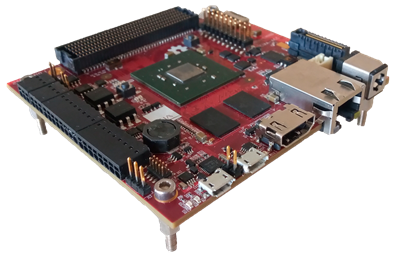
\includegraphics[width=\linewidth]{images/01-Introducción/ciaa.png}
        \caption{CIAA-ACC}
        \label{fig:intro_ciaa}
    \end{subfigure}
    \hfill
    \begin{subfigure}[b]{0.49\textwidth}
        \centering
        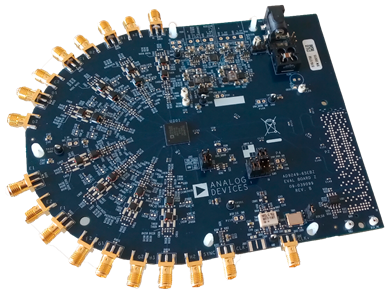
\includegraphics[width=\linewidth]{images/01-Introducción/ad.png}
        \caption{AD9249}
        \label{fig:intro_ad}
    \end{subfigure}
    \caption{Hardware donde se debe implementar el sistema a desarrollar.}
\end{figure}

El objetivo de este proyecto es el de realizar el estudio de las distintas técnicas de conformación digital de haz para definir la manera óptima de realizar una implementación bajo los requerimientos indicados, validando mediante simulaciones las decisiones de diseño adoptadas.

%\section{Organización de la tesis}